\documentclass[../analisi-dei-requisiti.tex]{subfiles}

\begin{document}
La presente sezione ha lo scopo di descrivere in maniera dettagliata, attraverso il linguaggio \glossario{UML}, le funzionalità offerte da \glossario{Stalker}.

\subsection{Attori dei casi d'uso}%
\label{sub:attori_casi_duso}

\subsubsection{Applicazione mobile}%
\label{subs:mobile_app}

\begin{figure}[H]
  \centering
  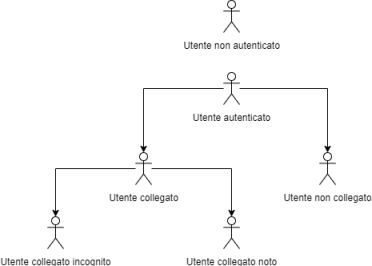
\includegraphics[width=100mm]{app_users.png}
  \caption{Utenti applicazione mobile}%
  \label{fig:usersapp}
\end{figure}

\subsubsection{Web application}%
\label{subs:web_application}

\begin{figure}[H]
  \centering
  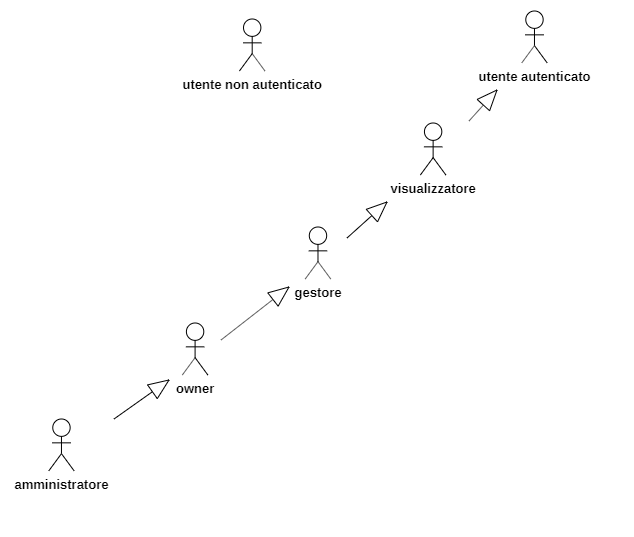
\includegraphics[width=100mm]{web_users.png}
  \caption{Utenti web application}%
  \label{fig:usersweb}
\end{figure}

\end{document}
